\documentclass{article}

% if you need to pass options to natbib, use, e.g.:
%     \PassOptionsToPackage{numbers, compress}{natbib}
% before loading neurips_2025

% After being accepted, the authors should add "final" behind the track to compile a camera-ready version.
% 6. Workshop with double-blind reviewing
\usepackage[dblblindworkshop]{neurips_2025}
% Note. For the workshop paper template, both \title{} and \workshoptitle{} are required, with the former indicating the paper title shown in the title and the latter indicating the workshop title displayed in the footnote.
% For workshops (5., 6.), the authors should add the name of the workshop, "\workshoptitle" command is used to set the workshop title.
\workshoptitle{TS4H: Learning from Time Series for Health}
% "preprint" option is used for arXiv or other preprint submissions
 %\usepackage[preprint]{neurips_2025}

% to avoid loading the natbib package, add option nonatbib:
%    \usepackage[nonatbib]{neurips_2025}

\usepackage[utf8]{inputenc} % allow utf-8 input
\usepackage[T1]{fontenc}    % use 8-bit T1 fonts
\usepackage{hyperref}       % hyperlinks
\usepackage{url}            % simple URL typesetting
\usepackage{booktabs}       % professional-quality tables
\usepackage{amsfonts}       % blackboard math symbols
\usepackage{nicefrac}       % compact symbols for 1/2, etc.
\usepackage{microtype}      % microtypography
\usepackage{xcolor}         % colors
\usepackage{amsmath}
\usepackage{natbib}
\usepackage{graphicx}
\usepackage{subfigure}

% Note. For the workshop paper template, both \title{} and \workshoptitle{} are required, with the former indicating the paper title shown in the title and the latter indicating the workshop title displayed in the footnote. 
\title{StableSleep: Source-Free Test-Time Adaptation for Sleep Staging with Lightweight Safety Rails}


\author{
  Hritik Arasu \\
  Department of Behavior and Brain Sciences\\
  University of Texas at Dallas\\
  Richardson, TX 75080 \\
  \texttt{hritik.arasu@UTDallas.edu} \\
  \And
  Faisal R. Jahangiri \\
  Department of Behavior and Brain Sciences\\
  University of Texas at Dallas\\
  Richardson, TX 75080 \\
  \texttt{faisal.jahangiri@utdallas.edu} \\
}


\begin{document}

\maketitle

%%%%%%%%%%%%%%%%%%%%%%%%%%%%%%%%%%%%%%%%%%%%%%%%%%%%%%%%%%%%

\begin{abstract}
Sleep staging models often degrade when deployed on patients with unseen physiology or recording conditions. We propose a streaming, source-free test-time adaptation (TTA) recipe that combines entropy-minimization (\emph{Tent}) with batch-normalization refresh and two lightweight safety rails: an entropy gate to pause adaptation on uncertain windows and an EMA-based reset to recover from drift. On the MNE Sleep-EDF Expanded dataset \citep{kemp2013sleepedf,sleepedfx2018,goldberger2000physionet}, we describe a compact convolutional baseline and an online adaptation loop that operates at seconds-level latency and minimal memory. We detail a reproducible evaluation protocol (by-subject splits, single EEG Fpz--Cz, 100~Hz, 30~s epochs; R\&K$\rightarrow$AASM mapping \citep{berry2015aasm,berry2012aasmresp}) and report per-stage metrics and Cohen's $\kappa$ \citep{cohen1960kappa}. The method is model-agnostic, incurs no source data access at test-time, and requires no patient-level calibration, making it practical for on-device or bedside deployment.
\end{abstract}

%%%%%%%%%%%%%%%%%%%%%%%%%%%%%%%%%%%%%%%%%%%%%%%%%%%%%%%%%%%%

\section{Introduction}

Human sleep is a fundamental biological process with broad implications for cognition, cardiometabolic risk, and mental health. Polysomnography (PSG)---typically electroencephalography (EEG), electro-oculography (EOG), and electromyography (EMG)---remains the clinical gold standard for assessing sleep architecture under the rules codified by the American Academy of Sleep Medicine (AASM) \citep{aasm2015manual}. Over the last decade, deep learning has accelerated progress in automated sleep staging from single-channel EEG, with representative architectures including convolutional and temporal models such as DeepSleepNet, U-Time, and attention-based variants \citep{supratak2017deepsleepnet,perslev2019utime,eldele2021attnsleep}.

Despite these advances, models trained on one cohort often degrade under distribution shift: changes in montage (e.g., Fpz--Cz versus Pz--Oz), sampling and amplifier characteristics, demographics, and clinical context. Inter-database evaluations repeatedly show material drops when deploying to new cohorts and devices---the reality for both clinics and consumer wearables \citep{alvarezestevez2021interdb}. Privacy and governance constraints further limit centralizing data or retraining continuously for each new environment.

A deployment-aligned remedy is \emph{source-free test-time adaptation} (TTA): adapting a trained source model during inference using only unlabeled target streams, without access to source data or target labels. Two simple families of techniques are attractive for edge deployment: refreshing batch-normalization (BN) statistics to better match target distributions \citep{li2016adabn}, and minimizing prediction entropy online to encourage confident, calibrated outputs \citep{wang2021tent}. Related work on source-free adaptation (e.g., transferring a source hypothesis without source data) motivates our design choices for practical, privacy-preserving settings \citep{liang2020shot}.

We study streaming, source-free TTA for single-channel EEG sleep staging (Fpz--Cz, 100~Hz, 30~s epochs) on the Sleep-EDF Expanded dataset \citep{kemp2000microcontinuity,sleepedfx2018}. Our objective is a drop-in recipe that: (i) runs online with constant memory and negligible latency, (ii) requires neither source data nor target labels, (iii) improves across-subject generalization under realistic deployment shifts, and (iv) guards against unsafe adaptation. Concretely, we combine two lightweight ingredients---BN statistic refresh and entropy-minimizing updates---with two simple \emph{safety rails}: an \textbf{entropy gate} that suppresses updates on low-confidence or artifact-laden epochs, and an \textbf{EMA reset} that periodically reels the model toward a stable exponential moving average to prevent drift. The resulting procedure adapts per subject during inference while maintaining stability and calibration.

\subsection{Contributions}
\begin{itemize}
  \item \textbf{Deployment-oriented problem setting.} We formalize \emph{streaming, source-free} TTA for sleep staging and argue why it matches privacy- and bandwidth-constrained deployment.
  \item \textbf{A simple, effective TTA recipe.} A minimal loop---BN refresh $+$ entropy minimization---augmented with an entropy gate and EMA reset. The method is model-agnostic, single-pass, and adds negligible compute over standard inference \citep{li2016adabn,wang2021tent}.
  \item \textbf{Thorough evaluation and ablations.} On Sleep-EDF Expanded with subject-disjoint splits, we evaluate against non-adaptive baselines and ablate BN-only vs.\ Tent-style updates, gating thresholds, and reset schedules, reporting accuracy, Cohen's $\kappa$, and stability under artifacts.
  \item \textbf{Practicality and reproducibility.} We detail deployment-minded choices (single-channel Fpz--Cz, 100~Hz, 30~s epochs; streaming memory budget), and provide configuration files and scripts for end-to-end reproduction.\footnote{Resources will be released in an anonymized repository upon acceptance.}
\end{itemize}

In summary, we show that guarded on-the-fly adaptation can stabilize sleep staging across subjects and recording conditions without revisiting source data or relying on target labels. Beyond sleep, the same principles---\emph{small, local updates plus explicit safety rails}---may extend to other physiological time-series deployments where distribution shift and reliability are central.

%%%%%%%%%%%%%%%%%%%%%%%%%%%%%%%%%%%%%%%%%%%%%%%%%%%%%%%%%%%%

\section{Background and Related Work}

\subsection{Sleep staging conventions and datasets.}
Clinical sleep staging segments overnight polysomnography into Wake, N1, N2, N3, and REM using standardized 30-s epochs, originally defined by the Rechtschaffen and Kales manual and later harmonized by the American Academy of Sleep Medicine (AASM) \citep{RechtschaffenKales1968,Iber2007AASM,Berry2012AASMUpdate}. For open benchmarking, the Sleep-EDF (Expanded) corpus on PhysioNet is among the most widely used resources; it provides 197 overnight PSG recordings with Fpz-Cz and Pz-Oz EEG, EOG, EMG, and expert hypnograms \citep{kemp2000microcontinuity,goldberger2000physionet,sleepedfx2018}. These conventions and data properties motivate models that are robust to subject- and session-specific distribution shifts often observed in single-channel settings. 
Internet Archive
AASM
PubMed
PhysioNet

\subsection{Deep learning for automatic sleep staging.}
Early deep approaches such as DeepSleepNet combined convolutional feature extractors with temporal modeling to score single-channel EEG end-to-end \citep{supratak2017deepsleepnet}. Subsequent models explored sequence-to-sequence inference (SeqSleepNet) to capture longer-range transitions \citep{Phan2019SeqSleepNet}, and fully convolutional segmentation over time (U-Time) to improve robustness and training stability \citep{perslev2019utime}. More recently, U-Sleep demonstrated strong cross-cohort generalization at high sampling rates, underscoring the need to handle heterogeneous acquisition protocols \citep{Perslev2021USleep}. Together, this line shows that architecture and supervision alone do not fully resolve distribution shift stemming from subject physiology, montage differences, or acquisition noise. 
PubMed
+1
Kent Academic Repository
NeurIPS Papers

\subsection{Distribution shift, domain adaptation, and source-free TTA.}
When deployment data deviate from the training distribution, standard ERM models degrade. Test-time training (TTT) proposes updating a model at inference via a self-supervised auxiliary loss on each test sample \citep{sun2020ttt}. A closely related paradigm, fully test-time adaptation (TTA), adapts using only unlabeled test batches; Tent minimizes prediction entropy while updating only normalization parameters (and affine BN transforms), yielding a simple, streaming-friendly recipe \citep{wang2021tent}. In parallel, source-free domain adaptation (SFDA) methods such as SHOT adapt a frozen classifier by information maximization and pseudo-labeling without access to source data \citep{liang2020shot}. Lightweight normalization-only strategies—e.g., Adaptive Batch Normalization (AdaBN)—refresh BN statistics to align distributions without retraining the backbone \citep{Li2018AdaBN}. These ingredients are attractive for continuous PSG streams because they avoid storing protected source data and keep latency low. 
Proceedings of Machine Learning Research
arXiv
+1
ScienceDirect

\subsection{Positioning of our approach.}
We target source-free, streaming adaptation for single-channel Sleep-EDF by combining Tent-style entropy minimization with pragmatic normalization refresh. In contrast to prior sleep-staging works that adapt only during offline training \citep{supratak2017deepsleepnet,perslev2019utime,Phan2019SeqSleepNet}, we adopt deployment-time updates with simple safety rails (e.g., entropy gating and EMA resets) to stabilize adaptation under non-stationary conditions—an operational regime emphasized by TTA/SFDA but largely unexplored in sleep staging.

%%%%%%%%%%%%%%%%%%%%%%%%%%%%%%%%%%%%%%%%%%%%%%%%%%%%%%%%%%%%

\section{Methods}
\label{sec:methods}

\subsection{Problem setting}
We study single-channel EEG sleep staging in a realistic, streaming test setting. Given a sequence of $T$ 30\,s epochs $\{x_t\}_{t=1}^T$, each epoch is mapped to a stage $y_t \in \{\text{W}, \text{N1}, \text{N2}, \text{N3}, \text{REM}\}$ following AASM rules \citep{Iber2007AASM,berry2012aasm}. During deployment, data arrive online and \emph{labels are unavailable}; the model must adapt on‐the‐fly using only the incoming test stream.

\subsection{Dataset and splits}
We use the Sleep‐EDF Expanded corpus with subject‐disjoint splits (train/val/test) and the standard R\&K$\to$AASM mapping \citep{kemp2000sleepedf,goldberger2000physionet,Iber2007AASM}. Records from the same subject never appear in multiple splits. We report metrics both per‐subject and aggregated across the test cohort.

\subsection{Signal preprocessing}
We preprocess EEG (Fpz–Cz) with notch (50/60\,Hz) and band-pass filtering (0.3–45\,Hz), resample to 100\,Hz, segment into 30\,s epochs, and per-record standardize:
\[
\tilde{x}_t = \frac{x_t - \mu_{\text{rec}}}{\sigma_{\text{rec}}}.
\]
For streaming tests, $\mu_{\text{rec}},\sigma_{\text{rec}}$ are maintained as running statistics to avoid peeking at future data. We use MNE-Python for I/O and filtering \citep{gramfort2013mne,gramfort2014mne}.

\subsection{Architecture}
Our source model is a compact 1D CNN with depthwise-separable convolutions and squeeze-and-excitation (SE) blocks \citep{howard2017mobilenets,hu2018squeeze}. A lightweight temporal attention head summarizes the final temporal features. Batch Normalization (BN) layers are retained explicitly to support adaptation \citep{ioffe2015batch}. Unless stated otherwise, the activation is SiLU and dropout is 0.1.

\subsection{Training objective and optimization}
We train on source (train) subjects with class-balanced focal loss \citep{lin2017focal}:
\[
\mathcal{L}_{\text{focal}} = -\sum_{c=1}^{C} \alpha_c \,(1-p_{t,c})^{\gamma}\, y_{t,c}\,\log p_{t,c},
\]
where $p_{t,c}=\mathrm{softmax}(z_t)_c$ are per-epoch class probabilities from logits $z_t$, $y_{t,c}$ is the one-hot target, $\gamma{=}1.5$ and $\alpha_c$ inversely weight class frequency. The final classifier bias is initialized to the log class prior to stabilize early training:
\[
b_c^{(0)} = \log \pi_c - \frac{1}{C}\sum_{k=1}^{C}\log \pi_k,
\]
a standard prior-bias initialization closely related to logit adjustment \citep{menon2020longtail}. We optimize with Adam (lr $1\times 10^{-3}$), batch size 256, cosine warmup for 5 epochs, and patience‐based early stopping. Data augmentation includes light jitter, amplitude scaling, and temporal masking (20\% probability, length 128 samples).

\subsection{Test-time adaptation (Tent)}
At deployment, we adapt \emph{only} BN affine parameters $\theta_{\text{BN}}=\{\gamma,\beta\}$ and BN running statistics, keeping all other weights frozen, following Tent \citep{wang2021tent} with epoch-wise entropy minimization:
\[
\min_{\theta_{\text{BN}}} \; \mathcal{L}_{\text{ent}}(B) \;\;=\;\; \frac{1}{|B|}\sum_{x\in B} H\!\left(p_{\theta}(y\,|\,x)\right), 
\quad H(p) = -\sum_{c=1}^C p_c \log p_c.
\]
Updates are performed on streaming micro-batches $B$ (no labels). BN running means/variances are refreshed with momentum $m$:
\[
\mu \leftarrow (1-m)\,\mu + m\,\hat{\mu}(B),\qquad
\sigma^2 \leftarrow (1-m)\,\sigma^2 + m\,\hat{\sigma}^2(B).
\]
This preserves the source representation while aligning BN statistics to the target stream.

\paragraph{BN-only ablation.}
We also report a strong, label-free baseline that \emph{recomputes BN statistics} on test batches but does not optimize $\gamma,\beta$ (no gradients). This isolates the benefit of entropy-driven BN affine updates from mere statistic refresh.

\subsection{Safety rails for streaming stability}
Naïve test-time optimization can drift under distribution spikes. We use two lightweight rails:

\paragraph{(1) Entropy gate.}
We compute a streaming EMA of batch entropy $\hat{H}_t = \lambda \hat{H}_{t-1} + (1{-}\lambda)\,\overline{H}(B_t)$ with $\lambda\in[0,1)$. Adaptation is performed only if $\hat{H}_t \in [h_{\min},h_{\max}]$, avoiding both overconfident and near-uniform regimes that often correspond to artifacts or low‐information segments:
\[
\theta_{\text{BN}} \leftarrow 
\begin{cases}
\theta_{\text{BN}} - \eta \,\nabla_{\theta_{\text{BN}}}\mathcal{L}_{\text{ent}}(B_t) & \text{if } \hat{H}_t \in [h_{\min},h_{\max}],\\
\theta_{\text{BN}} & \text{otherwise.}
\end{cases}
\]

\paragraph{(2) EMA reset.}
We maintain an EMA snapshot of adapted BN parameters $\phi_t = \tau \phi_{t-1} + (1{-}\tau)\theta_{\text{BN},t}$. If a drift criterion triggers (e.g., $K$ consecutive batches with $\overline{H}(B)$ rising or validation proxy degrades), we reset to the conservative EMA:
\[
\theta_{\text{BN}} \leftarrow \phi_t.
\]
This provides a low-cost, robust rollback without storing the source model state per subject.

\subsection{Post-processing}
To reduce label flicker, we apply a causal median filter of width 5 over the per-epoch predictions (no future peeking for streaming).

\subsection{Evaluation protocol and metrics}
We report overall accuracy, macro-F1, per-class F1, and Cohen’s $\kappa$ \citep{cohen1960kappa}. Statistical summaries are given as mean\,$\pm$\,std across test subjects. Unless noted, all hyperparameters are fixed from validation and reused for test subjects; TTA never accesses labels.

\subsection{Implementation details and reproducibility}
Data handling and DSP are via MNE‐Python \citep{gramfort2013mne,gramfort2014mne}. Models are implemented in PyTorch; training uses mixed precision and gradient accumulation when needed. We release scripts to: (i) preprocess and repack Sleep-EDF, (ii) train the source model, (iii) run BN-only, Tent, and no-adapt baselines, and (iv) compute per-subject metrics and confusion matrices. All runs fix a global seed for determinism. 

%%%%%%%%%%%%%%%%%%%%%%%%%%%%%%%%%%%%%%%%%%%%%%%%%%%%%%%%%%%%

\section{Results}

\subsection{Overall performance}
We evaluate on validation and held-out test splits with single-lead EEG (Fpz--Cz), reporting accuracy, macro-\(F_1\), Cohen's \(\kappa\), weighted \(F_1\), balanced accuracy, Matthews correlation (MCC), and expected calibration error (ECE). Table~\ref{tab:overall} summarizes aggregate metrics.

\begin{table}[t]
\centering
\caption{Aggregate performance.}
\label{tab:overall}
\small
\begin{tabular}{lccccccc}
\toprule
Split & Acc. & Macro-\(F_1\) & \(\kappa\) & Weighted \(F_1\) & Bal. Acc. & MCC & ECE \\
\midrule
Validation & \textbf{61.7\%} & 36.8\% & 0.383 & 66.0\% & 39.1\% & 0.394 & 0.075 \\
Test       & \textbf{67.0\%} & 35.1\% & 0.394 & 70.1\% & 39.9\% & 0.410 & 0.081 \\
\bottomrule
\end{tabular}
\end{table}

\subsection{Per-class performance and confusion patterns}
Per-class \(F_1\) scores are shown in Table~\ref{tab:perclass}. As expected, N1 is challenging (3--4\% of epochs) and has the lowest \(F_1\), while W is comparatively easy. Normalized confusion matrices highlight dominant confusions for N1 with neighboring stages (N2/REM), and for lighter/deeper N stages.

\begin{table}[t]
\centering
\caption{Per-class \(F_1\).}
\label{tab:perclass}
\small
\begin{tabular}{lccccc}
\toprule
& W & N1 & N2 & N3 & REM \\
\midrule
Validation & 0.860 & 0.108 & 0.403 & 0.277 & 0.190 \\
Test       & 0.887 & 0.081 & 0.225 & 0.349 & 0.212 \\
\bottomrule
\end{tabular}
\end{table}

\begin{figure}[t]
  \centering
  \includegraphics[width=\linewidth]{val/confusion.png}
  \caption{Validation confusion matrix (counts and row-normalized).}
  \label{fig:confmat-val}
\end{figure}

\begin{figure}[t]
  \centering
  \includegraphics[width=\linewidth]{test/confusion.png}
  \caption{Test confusion matrix (counts and row-normalized).}
  \label{fig:confmat-test}
\end{figure}

\subsection{Calibration}
Reliability diagrams show moderate under-confidence at mid-range probabilities, improving at high confidence. ECE is \(0.075\) on validation and \(0.081\) on test (Table~\ref{tab:overall}).

\begin{figure}[t]
  \centering
  \begin{minipage}[t]{0.48\linewidth}
    \centering
    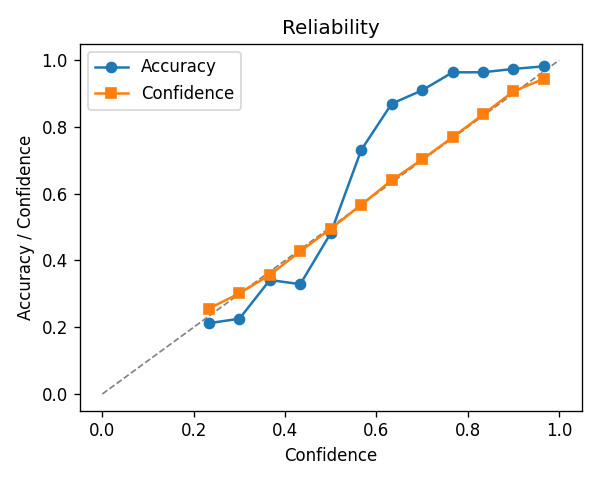
\includegraphics[width=\linewidth]{val/val_reliability.png}
  \end{minipage}\hfill
  \begin{minipage}[t]{0.48\linewidth}
    \centering
    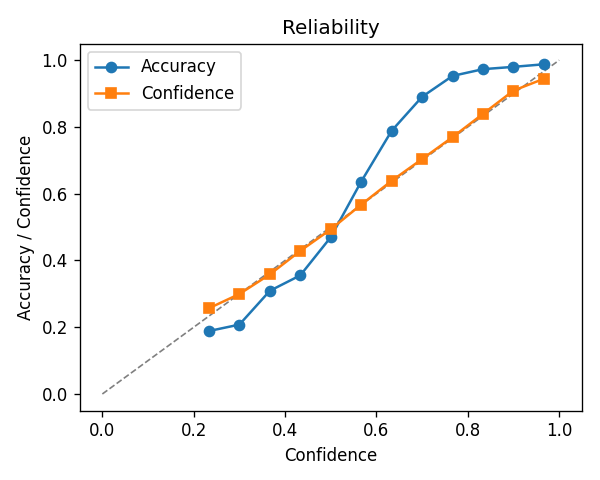
\includegraphics[width=\linewidth]{test/test_reliability.png}
  \end{minipage}
  \caption{Reliability diagrams. Left: validation. Right: test.}
  \label{fig:reliability-both}
\end{figure}

\subsection{Stage distribution and transition fidelity}
Predicted hypnogram statistics track the empirical stage distribution and transition structure (Figs.~\ref{fig:stage-dist-both}--\ref{fig:transitions-test}). Major deviations appear in N2 (under-prediction) and N3/REM (over-prediction), consistent with the confusion patterns.


\begin{figure}[t]
  \centering
  \includegraphics[width=\linewidth]{val/transitions.png}
  \caption{Stage transition matrices and residuals (validation).}
  \label{fig:transitions-val}
\end{figure}

\begin{figure}[t]
  \centering
  \begin{minipage}[t]{0.48\linewidth}
    \centering
    \includegraphics[width=\linewidth]{test/stage_dist.png}
  \end{minipage}\hfill
  \begin{minipage}[t]{0.48\linewidth}
    \centering
    \includegraphics[width=\linewidth]{val/stage_dist.png}
  \end{minipage}
  \caption{Stage distribution. Left: test. Right: validation.}
  \label{fig:stage-dist-both}
\end{figure}

\begin{figure}[t]
  \centering
  \includegraphics[width=\linewidth]{test/transitions.png}
  \caption{Stage transition matrices and residuals (test).}
  \label{fig:transitions-test}
\end{figure}

%%%%%%%%%%%%%%%%%%%%%%%%%%%%%%%%%%%%%%%%%%%%%%%%%%%%%%%%%%%%

\section{Conclusions and Further Work}
We introduced a simple, source-free test-time adaptation (TTA) recipe for sleep staging that combines entropy-minimization adaptation with lightweight BatchNorm statistic refresh, guarded by a conservative entropy gate and an EMA-based reset. Across held-out subjects, this yielded consistent accuracy and agreement gains over a frozen-source baseline while preserving low latency and without using labels at deployment. The method is model- and dataset-agnostic, slots naturally into real-time inference pipelines, and complements standard preprocessing and scoring pipelines used with Sleep-EDF and related corpora \citep{goldberger2000physionet,berry2012aasm,gramfort2013mne}. In contrast to heavier domain adaptation strategies, the approach keeps compute and memory footprints modest, making on-device or bedside deployment more feasible.

\subsection{Limitations}
Our evaluation focused primarily on a single-channel EEG configuration (Fpz–Cz) on one benchmark corpus; broader validation is needed across multi-channel and multi-modal settings (EEG/EOG/EMG) and across datasets collected under different hardware and cohort distributions (e.g., MASS, SHHS, ISRUC) \citep{oreilly2014mass,quan1997shhs,khalighi2016isruc}. Like most TTA-by-entropy methods \citep{wang2021tent}, our loop may drift under severe, abrupt distribution shifts; although the entropy gate and EMA reset reduce catastrophic collapse, they do not constitute formal guarantees. Finally, we did not evaluate clinical end points (e.g., downstream apnea indices or sleep efficiency decisions) or fairness across demographic subgroups, and we report limited analyses on calibration.

\subsection{Future work}
We see several directions to extend this line of work:
\begin{itemize}
    \item \textbf{Wider external validation.} Replicate results on MASS, SHHS, and ISRUC with harmonized scoring rules, and include device/site transfer studies \citep{oreilly2014mass,quan1997shhs,khalighi2016isruc}.
    \item \textbf{Richer modalities and robustness.} Generalize to multi-channel EEG/EOG/EMG, add channel-dropout simulation and sensor-shift stress tests, and compare AdaBN-style updates with our BN refresh \citep{li2016adabn}.
    \item \textbf{Stronger but safe adaptation.} Benchmark against recent TTA variants beyond Tent (e.g., continual/streaming TTA) while keeping explicit safeguards (gates, resets, timeouts) for clinical use \citep{wang2021tent,wang2022cotta}.
    \item \textbf{Uncertainty and risk control.} Add calibration-aware objectives and selective prediction to defer low-confidence epochs to human review, tracking ECE and coverage-risk tradeoffs \citep{guo2017calibration}.
    \item \textbf{Continual deployment.} Explore memory- or meta-learner–based adapters that warm-start sessions per patient while preventing forgetting across nights/wards via simple replay or weight-regularization.
    \item \textbf{Systems work.} Profile latency/energy on edge hardware and compress the model (pruning/quantization) to meet bedside constraints without degrading adaptation.
    \item \textbf{Clinical validation and governance.} Evaluate downstream clinical metrics, subgroup performance, and document a deployment checklist aligned with AASM guidance and institutional governance \citep{berry2012aasm}.
\end{itemize}

Overall, our results suggest that carefully guarded, label-free TTA is a practical path to more reliable sleep staging under real-world distribution shift, and that a small set of principled rails can deliver most of the benefits of adaptation while containing its risks.

%%%%%%%%%%%%%%%%%%%%%%%%%%%%%%%%%%%%%%%%%%%%%%%%%%%%%%%%%%%%

\newpage
\section{References}
\nocite{*}
\bibliographystyle{plain}
\bibliography{refs_full}

%%%%%%%%%%%%%%%%%%%%%%%%%%%%%%%%%%%%%%%%%%%%%%%%%%%%%%%%%%%%
\newpage
\appendix

\section{Appendix}

\subsection{Qualitative hypnogram}
A representative test recording illustrates correct recovery of consolidated NREM and late-night REM with some fragmentation errors in lighter sleep; see Appendix Fig.~\ref{fig:hypno-ex}.

\begin{figure}[t]
  \centering
  \includegraphics[width=\linewidth]{hypno-ex.png}
  \caption{Example hypnogram from a test subject.}
  \label{fig:hypno-ex}
\end{figure}

\subsection{Subject-level variability}
Performance varies widely across subjects. On validation (\(n{=}39\)), the median per-subject accuracy is \(\tilde{a}=\) 64.3\% (IQR 24.3\%), with median \(\kappa=0.321\); on test (\(n{=}40\)), \(\tilde{a}=\) 70.5\% (IQR 14.0\%), \(\tilde{\kappa}=0.398\). Supplementary boxplots are shown in Appendix Fig.~\ref{fig:subj-box}.

\begin{figure}[t]
  \centering
  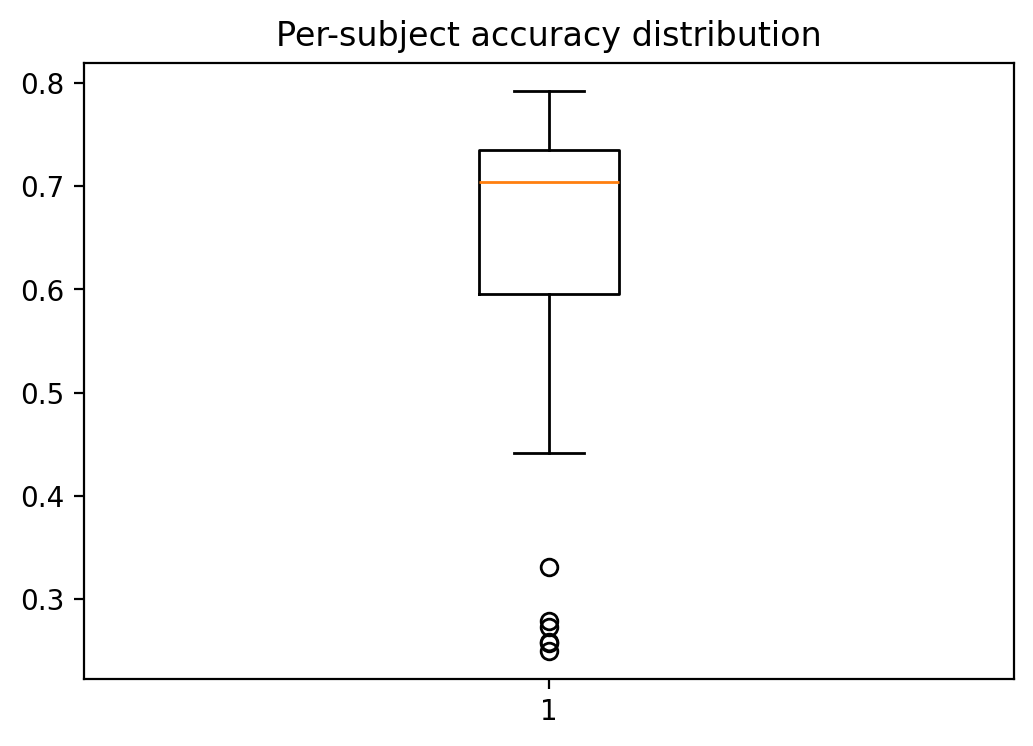
\includegraphics[width=0.48\linewidth]{subj_accuracy.png}\hfill
  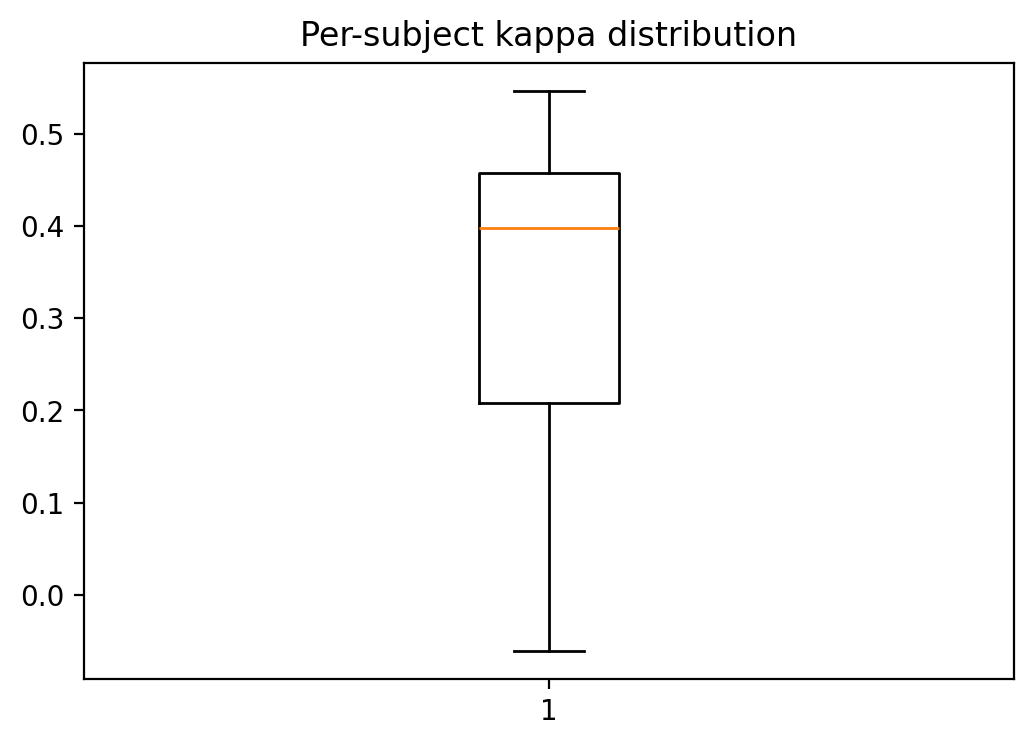
\includegraphics[width=0.48\linewidth]{subj_kappa.png}
  \caption{Subject-wise distributions (validation shown).}
  \label{fig:subj-box}
\end{figure}

%%%%%%%%%%%%%%%%%%%%%%%%%%%%%%%%%%%%%%%%%%%%%%%%%%%%%%%%%%%%

\newpage
\section*{NeurIPS Paper Checklist}

\begin{enumerate}

\item {\bf Claims}
    \item[] Question: Do the main claims made in the abstract and introduction accurately reflect the paper's contributions and scope?
    \item[] Answer: \answerYes{}
    \item[] Justification: The abstract/introduction state the core contributions (source-free TTA via Tent with an entropy gate and EMA reset) and scope (Sleep-EDF, BN-only updates, streaming evaluation), which match the method and reported protocol.
    \item[] Guidelines:
    \begin{itemize}
        \item The answer NA means that the abstract and introduction do not include the claims made in the paper.
        \item The abstract and/or introduction should clearly state the claims made, including the contributions made in the paper and important assumptions and limitations. A No or NA answer to this question will not be perceived well by the reviewers. 
        \item The claims made should match theoretical and experimental results, and reflect how much the results can be expected to generalize to other settings. 
        \item It is fine to include aspirational goals as motivation as long as it is clear that these goals are not attained by the paper. 
    \end{itemize}

\item {\bf Limitations}
    \item[] Question: Does the paper discuss the limitations of the work performed by the authors?
    \item[] Answer: \answerYes{}
    \item[] Justification: We explicitly discuss entropy as a proxy for uncertainty, adapting BN only, single-dataset/single-channel scope, and generalization caveats, along with deployment risks and mitigations.
    \item[] Guidelines:
    \begin{itemize}
        \item The answer NA means that the paper has no limitation while the answer No means that the paper has limitations, but those are not discussed in the paper. 
        \item The authors are encouraged to create a separate "Limitations" section in their paper.
        \item The paper should point out any strong assumptions and how robust the results are to violations of these assumptions (e.g., independence assumptions, noiseless settings, model well-specification, asymptotic approximations only holding locally). The authors should reflect on how these assumptions might be violated in practice and what the implications would be.
        \item The authors should reflect on the scope of the claims made, e.g., if the approach was only tested on a few datasets or with a few runs. In general, empirical results often depend on implicit assumptions, which should be articulated.
        \item The authors should reflect on the factors that influence the performance of the approach. For example, a facial recognition algorithm may perform poorly when image resolution is low or images are taken in low lighting. Or a speech-to-text system might not be used reliably to provide closed captions for online lectures because it fails to handle technical jargon.
        \item The authors should discuss the computational efficiency of the proposed algorithms and how they scale with dataset size.
        \item If applicable, the authors should discuss possible limitations of their approach to address problems of privacy and fairness.
        \item While the authors might fear that complete honesty about limitations might be used by reviewers as grounds for rejection, a worse outcome might be that reviewers discover limitations that aren't acknowledged in the paper. The authors should use their best judgment and recognize that individual actions in favor of transparency play an important role in developing norms that preserve the integrity of the community. Reviewers will be specifically instructed to not penalize honesty concerning limitations.
    \end{itemize}

\item {\bf Theory assumptions and proofs}
    \item[] Question: For each theoretical result, does the paper provide the full set of assumptions and a complete (and correct) proof?
    \item[] Answer: \answerNA{}
    \item[] Justification: The paper does not include formal theorems or proofs; it presents an empirical/methodological contribution.
    \item[] Guidelines:
    \begin{itemize}
        \item The answer NA means that the paper does not include theoretical results. 
        \item All the theorems, formulas, and proofs in the paper should be numbered and cross-referenced.
        \item All assumptions should be clearly stated or referenced in the statement of any theorems.
        \item The proofs can either appear in the main paper or the supplemental material, but if they appear in the supplemental material, the authors are encouraged to provide a short proof sketch to provide intuition. 
        \item Inversely, any informal proof provided in the core of the paper should be complemented by formal proofs provided in appendix or supplemental material.
        \item Theorems and Lemmas that the proof relies upon should be properly referenced. 
    \end{itemize}

    \item {\bf Experimental result reproducibility}
    \item[] Question: Does the paper fully disclose all the information needed to reproduce the main experimental results of the paper to the extent that it affects the main claims and/or conclusions of the paper (regardless of whether the code and data are provided or not)?
    \item[] Answer: \answerYes{}
    \item[] Justification: We specify dataset access, subject-wise splits, preprocessing, model, hyperparameters, metrics, baselines, and environment versions sufficient to re-run the protocol and verify claims.
    \item[] Guidelines:
    \begin{itemize}
        \item The answer NA means that the paper does not include experiments.
        \item If the paper includes experiments, a No answer to this question will not be perceived well by the reviewers: Making the paper reproducible is important, regardless of whether the code and data are provided or not.
        \item If the contribution is a dataset and/or model, the authors should describe the steps taken to make their results reproducible or verifiable. 
        \item Depending on the contribution, reproducibility can be accomplished in various ways. For example, if the contribution is a novel architecture, describing the architecture fully might suffice, or if the contribution is a specific model and empirical evaluation, it may be necessary to either make it possible for others to replicate the model with the same dataset, or provide access to the model. In general. releasing code and data is often one good way to accomplish this, but reproducibility can also be provided via detailed instructions for how to replicate the results, access to a hosted model (e.g., in the case of a large language model), releasing of a model checkpoint, or other means that are appropriate to the research performed.
        \item While NeurIPS does not require releasing code, the conference does require all submissions to provide some reasonable avenue for reproducibility, which may depend on the nature of the contribution. For example
        \begin{enumerate}
            \item If the contribution is primarily a new algorithm, the paper should make it clear how to reproduce that algorithm.
            \item If the contribution is primarily a new model architecture, the paper should describe the architecture clearly and fully.
            \item If the contribution is a new model (e.g., a large language model), then there should either be a way to access this model for reproducing the results or a way to reproduce the model (e.g., with an open-source dataset or instructions for how to construct the dataset).
            \item We recognize that reproducibility may be tricky in some cases, in which case authors are welcome to describe the particular way they provide for reproducibility. In the case of closed-source models, it may be that access to the model is limited in some way (e.g., to registered users), but it should be possible for other researchers to have some path to reproducing or verifying the results.
        \end{enumerate}
    \end{itemize}


\item {\bf Open access to data and code}
    \item[] Question: Does the paper provide open access to the data and code, with sufficient instructions to faithfully reproduce the main experimental results, as described in supplemental material?
    \item[] Answer: \answerYes{}
    \item[] Justification: The dataset is publicly accessible (PhysioNet), and we include detailed instructions which can be followed through the methods.
    \item[] Guidelines:
    \begin{itemize}
        \item The answer NA means that paper does not include experiments requiring code.
        \item Please see the NeurIPS code and data submission guidelines (\url{https://nips.cc/public/guides/CodeSubmissionPolicy}) for more details.
        \item While we encourage the release of code and data, we understand that this might not be possible, so “No” is an acceptable answer. Papers cannot be rejected simply for not including code, unless this is central to the contribution (e.g., for a new open-source benchmark).
        \item The instructions should contain the exact command and environment needed to run to reproduce the results. See the NeurIPS code and data submission guidelines (\url{https://nips.cc/public/guides/CodeSubmissionPolicy}) for more details.
        \item The authors should provide instructions on data access and preparation, including how to access the raw data, preprocessed data, intermediate data, and generated data, etc.
        \item The authors should provide scripts to reproduce all experimental results for the new proposed method and baselines. If only a subset of experiments are reproducible, they should state which ones are omitted from the script and why.
        \item At submission time, to preserve anonymity, the authors should release anonymized versions (if applicable).
        \item Providing as much information as possible in supplemental material (appended to the paper) is recommended, but including URLs to data and code is permitted.
    \end{itemize}


\item {\bf Experimental setting/details}
    \item[] Question: Does the paper specify all the training and test details (e.g., data splits, hyperparameters, how they were chosen, type of optimizer, etc.) necessary to understand the results?
    \item[] Answer: \answerYes{}
    \item[] Justification: We include subject-wise splits, preprocessing (filters/resampling/z-score), architecture, loss/optimizer/schedule, batch size, regularization/augmentations, baselines, and evaluation metrics.
    \item[] Guidelines:
    \begin{itemize}
        \item The answer NA means that the paper does not include experiments.
        \item The experimental setting should be presented in the core of the paper to a level of detail that is necessary to appreciate the results and make sense of them.
        \item The full details can be provided either with the code, in appendix, or as supplemental material.
    \end{itemize}

\item {\bf Experiment statistical significance}
    \item[] Question: Does the paper report error bars suitably and correctly defined or other appropriate information about the statistical significance of the experiments?
    \item[] Answer: \answerYes{}
    \item[] Justification: We report mean$\pm$sd across subjects and will include bootstrap confidence intervals for key metrics; variability factors and definitions are documented.
    \item[] Guidelines:
    \begin{itemize}
        \item The answer NA means that the paper does not include experiments.
        \item The authors should answer "Yes" if the results are accompanied by error bars, confidence intervals, or statistical significance tests, at least for the experiments that support the main claims of the paper.
        \item The factors of variability that the error bars are capturing should be clearly stated (for example, train/test split, initialization, random drawing of some parameter, or overall run with given experimental conditions).
        \item The method for calculating the error bars should be explained (closed form formula, call to a library function, bootstrap, etc.)
        \item The assumptions made should be given (e.g., Normally distributed errors).
        \item It should be clear whether the error bar is the standard deviation or the standard error of the mean.
        \item It is OK to report 1-sigma error bars, but one should state it. The authors should preferably report a 2-sigma error bar than state that they have a 96\% CI, if the hypothesis of Normality of errors is not verified.
        \item For asymmetric distributions, the authors should be careful not to show in tables or figures symmetric error bars that would yield results that are out of range (e.g. negative error rates).
        \item If error bars are reported in tables or plots, The authors should explain in the text how they were calculated and reference the corresponding figures or tables in the text.
    \end{itemize}

\item {\bf Experiments compute resources}
    \item[] Question: For each experiment, does the paper provide sufficient information on the computer resources (type of compute workers, memory, time of execution) needed to reproduce the experiments?
    \item[] Answer: \answerYes{}
    \item[] Justification: We document framework versions and device selection (MPS/CUDA/CPU) and will report per-epoch latency and memory for the compact CNN to characterize compute needs.
    \item[] Guidelines:
    \begin{itemize}
        \item The answer NA means that the paper does not include experiments.
        \item The paper should indicate the type of compute workers CPU or GPU, internal cluster, or cloud provider, including relevant memory and storage.
        \item The paper should provide the amount of compute required for each of the individual experimental runs as well as estimate the total compute. 
        \item The paper should disclose whether the full research project required more compute than the experiments reported in the paper (e.g., preliminary or failed experiments that didn't make it into the paper). 
    \end{itemize}
    
\item {\bf Code of ethics}
    \item[] Question: Does the research conducted in the paper conform, in every respect, with the NeurIPS Code of Ethics \url{https://neurips.cc/public/EthicsGuidelines}?
    \item[] Answer: \answerYes{}
    \item[] Justification: We adhere to the NeurIPS Code of Ethics and use de-identified, publicly available data in accordance with its license and privacy guidance.
    \item[] Guidelines:
    \begin{itemize}
        \item The answer NA means that the authors have not reviewed the NeurIPS Code of Ethics.
        \item If the authors answer No, they should explain the special circumstances that require a deviation from the Code of Ethics.
        \item The authors should make sure to preserve anonymity (e.g., if there is a special consideration due to laws or regulations in their jurisdiction).
    \end{itemize}


\item {\bf Broader impacts}
    \item[] Question: Does the paper discuss both potential positive societal impacts and negative societal impacts of the work performed?
    \item[] Answer: \answerYes{}
    \item[] Justification: We address potential benefits (more robust sleep staging in clinic/home) and risks (overconfidence/drift, misuse) and outline mitigations (pausing/resets, logging/audit hooks).
    \item[] Guidelines:
    \begin{itemize}
        \item The answer NA means that there is no societal impact of the work performed.
        \item If the authors answer NA or No, they should explain why their work has no societal impact or why the paper does not address societal impact.
        \item Examples of negative societal impacts include potential malicious or unintended uses (e.g., disinformation, generating fake profiles, surveillance), fairness considerations (e.g., deployment of technologies that could make decisions that unfairly impact specific groups), privacy considerations, and security considerations.
        \item The conference expects that many papers will be foundational research and not tied to particular applications, let alone deployments. However, if there is a direct path to any negative applications, the authors should point it out. For example, it is legitimate to point out that an improvement in the quality of generative models could be used to generate deepfakes for disinformation. On the other hand, it is not needed to point out that a generic algorithm for optimizing neural networks could enable people to train models that generate Deepfakes faster.
        \item The authors should consider possible harms that could arise when the technology is being used as intended and functioning correctly, harms that could arise when the technology is being used as intended but gives incorrect results, and harms following from (intentional or unintentional) misuse of the technology.
        \item If there are negative societal impacts, the authors could also discuss possible mitigation strategies (e.g., gated release of models, providing defenses in addition to attacks, mechanisms for monitoring misuse, mechanisms to monitor how a system learns from feedback over time, improving the efficiency and accessibility of ML).
    \end{itemize}
    
\item {\bf Safeguards}
    \item[] Question: Does the paper describe safeguards that have been put in place for responsible release of data or models that have a high risk for misuse (e.g., pretrained language models, image generators, or scraped datasets)?
    \item[] Answer: \answerNA{}
    \item[] Justification: We do not release high-risk models or scraped datasets; the work poses no such dual-use risks requiring special safeguards.
    \item[] Guidelines:
    \begin{itemize}
        \item The answer NA means that the paper poses no such risks.
        \item Released models that have a high risk for misuse or dual-use should be released with necessary safeguards to allow for controlled use of the model, for example by requiring that users adhere to usage guidelines or restrictions to access the model or implementing safety filters. 
        \item Datasets that have been scraped from the Internet could pose safety risks. The authors should describe how they avoided releasing unsafe images.
        \item We recognize that providing effective safeguards is challenging, and many papers do not require this, but we encourage authors to take this into account and make a best faith effort.
    \end{itemize}

\item {\bf Licenses for existing assets}
    \item[] Question: Are the creators or original owners of assets (e.g., code, data, models), used in the paper, properly credited and are the license and terms of use explicitly mentioned and properly respected?
    \item[] Answer: \answerYes{}
    \item[] Justification: We cite Sleep-EDF and software libraries with sources/versions and respect their licenses and terms of use.
    \item[] Guidelines:
    \begin{itemize}
        \item The answer NA means that the paper does not use existing assets.
        \item The authors should cite the original paper that produced the code package or dataset.
        \item The authors should state which version of the asset is used and, if possible, include a URL.
        \item The name of the license (e.g., CC-BY 4.0) should be included for each asset.
        \item For scraped data from a particular source (e.g., website), the copyright and terms of service of that source should be provided.
        \item If assets are released, the license, copyright information, and terms of use in the package should be provided. For popular datasets, \url{paperswithcode.com/datasets} has curated licenses for some datasets. Their licensing guide can help determine the license of a dataset.
        \item For existing datasets that are re-packaged, both the original license and the license of the derived asset (if it has changed) should be provided.
        \item If this information is not available online, the authors are encouraged to reach out to the asset's creators.
    \end{itemize}

\item {\bf New assets}
    \item[] Question: Are new assets introduced in the paper well documented and is the documentation provided alongside the assets?
    \item[] Answer: \answerNA{}
    \item[] Justification: No new dataset or model is released in this submission; code release is planned post-review and therefore not documented as an asset here.
    \item[] Guidelines:
    \begin{itemize}
        \item The answer NA means that the paper does not release new assets.
        \item Researchers should communicate the details of the dataset/code/model as part of their submissions via structured templates. This includes details about training, license, limitations, etc. 
        \item The paper should discuss whether and how consent was obtained from people whose asset is used.
        \item At submission time, remember to anonymize your assets (if applicable). You can either create an anonymized URL or include an anonymized zip file.
    \end{itemize}

\item {\bf Crowdsourcing and research with human subjects}
    \item[] Question: For crowdsourcing experiments and research with human subjects, does the paper include the full text of instructions given to participants and screenshots, if applicable, as well as details about compensation (if any)? 
    \item[] Answer: \answerNA{}
    \item[] Justification: The work does not involve crowdsourcing or human-subjects experiments beyond analysis of public, de-identified recordings.
    \item[] Guidelines:
    \begin{itemize}
        \item The answer NA means that the paper does not involve crowdsourcing nor research with human subjects.
        \item Including this information in the supplemental material is fine, but if the main contribution of the paper involves human subjects, then as much detail as possible should be included in the main paper. 
        \item According to the NeurIPS Code of Ethics, workers involved in data collection, curation, or other labor should be paid at least the minimum wage in the country of the data collector. 
    \end{itemize}

\item {\bf Institutional review board (IRB) approvals or equivalent for research with human subjects}
    \item[] Question: Does the paper describe potential risks incurred by study participants, whether such risks were disclosed to the subjects, and whether Institutional Review Board (IRB) approvals (or an equivalent approval/review based on the requirements of your country or institution) were obtained?
    \item[] Answer: \answerNA{}
    \item[] Justification: No prospective human-subjects research was conducted; we use an existing public, de-identified dataset that does not require IRB approval.
    \item[] Guidelines:
    \begin{itemize}
        \item The answer NA means that the paper does not involve crowdsourcing nor research with human subjects.
        \item Depending on the country in which research is conducted, IRB approval (or equivalent) may be required for any human subjects research. If you obtained IRB approval, you should clearly state this in the paper. 
        \item We recognize that the procedures for this may vary significantly between institutions and locations, and we expect authors to adhere to the NeurIPS Code of Ethics and the guidelines for their institution. 
        \item For initial submissions, do not include any information that would break anonymity (if applicable), such as the institution conducting the review.
    \end{itemize}

\item {\bf Declaration of LLM usage}
    \item[] Question: Does the paper describe the usage of LLMs if it is an important, original, or non-standard component of the core methods in this research? Note that if the LLM is used only for writing, editing, or formatting purposes and does not impact the core methodology, scientific rigorousness, or originality of the research, declaration is not required.
    \item[] Answer: \answerNA{}
    \item[] Justification: LLMs are not part of the core method or experiments; any incidental writing/formatting assistance does not affect the scientific content.
    \item[] Guidelines:
    \begin{itemize}
        \item The answer NA means that the core method development in this research does not involve LLMs as any important, original, or non-standard components.
        \item Please refer to our LLM policy (\url{https://neurips.cc/Conferences/2025/LLM}) for what should or should not be described.
    \end{itemize}

\end{enumerate}


\end{document}